\section{Конструкторский раздел}

\subsection{Диаграмма вариантов использования}

\subsection{Блок-схема работы сервера}
На рисунке \ref{fig:serverScheme} предоставлена блок-схема начала работы сервера и алгоритма обработки запросов пользователей.

\begin{figure}[hbtp]
	\centering
	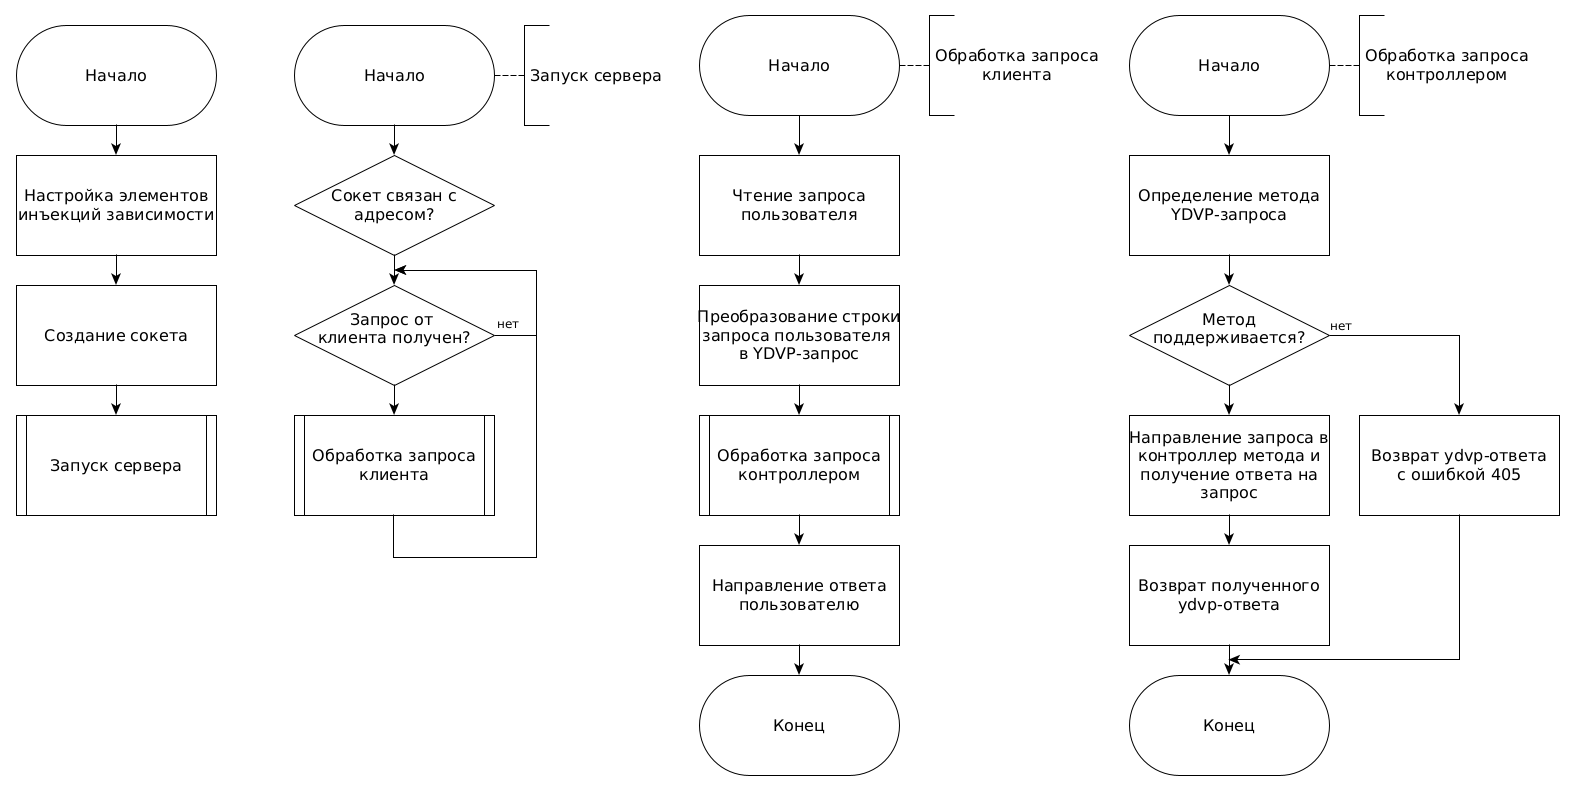
\includegraphics[width=\textwidth]{img/serverScheme.png}
	\caption{Блок-схема работы сервера приложения. }
	\label{fig:serverScheme}
\end{figure}

\subsection{Описание YDVP-протокола}
На основе существующего стандарта HTTP в данном подразделе описывается структура реализуемого YDVP-протокола.

YDVP-запрос включает в себя три компонента:
\begin{itemize}[leftmargin=1.6\parindent]
\item стартовую строку (определяющей тип сообщения);
\item заголовки (характеризующих тело сообщения, параметры передачи и т.д.);
\item тело (данные сообщения).
\end{itemize}

И так далее по списку, грубо говоря, только копируем...
Обязательно говорим о том, что в нашем протоколе потребуется только поддержка GET и POST методов, а также пара слов о том, что текущая версия 0.1

\pagebreak